%==============================================================================
% Figure: Dimensional Folding Visualization
% Purpose: Illustrate origami dimension concept from Genesis framework
% Chapter: Ch13 - Genesis Framework: Dimensional Folding and Origami Principles
% Type: Conceptual diagram / Visual metaphor
%==============================================================================

\begin{figure}[htbp]
  \centering
  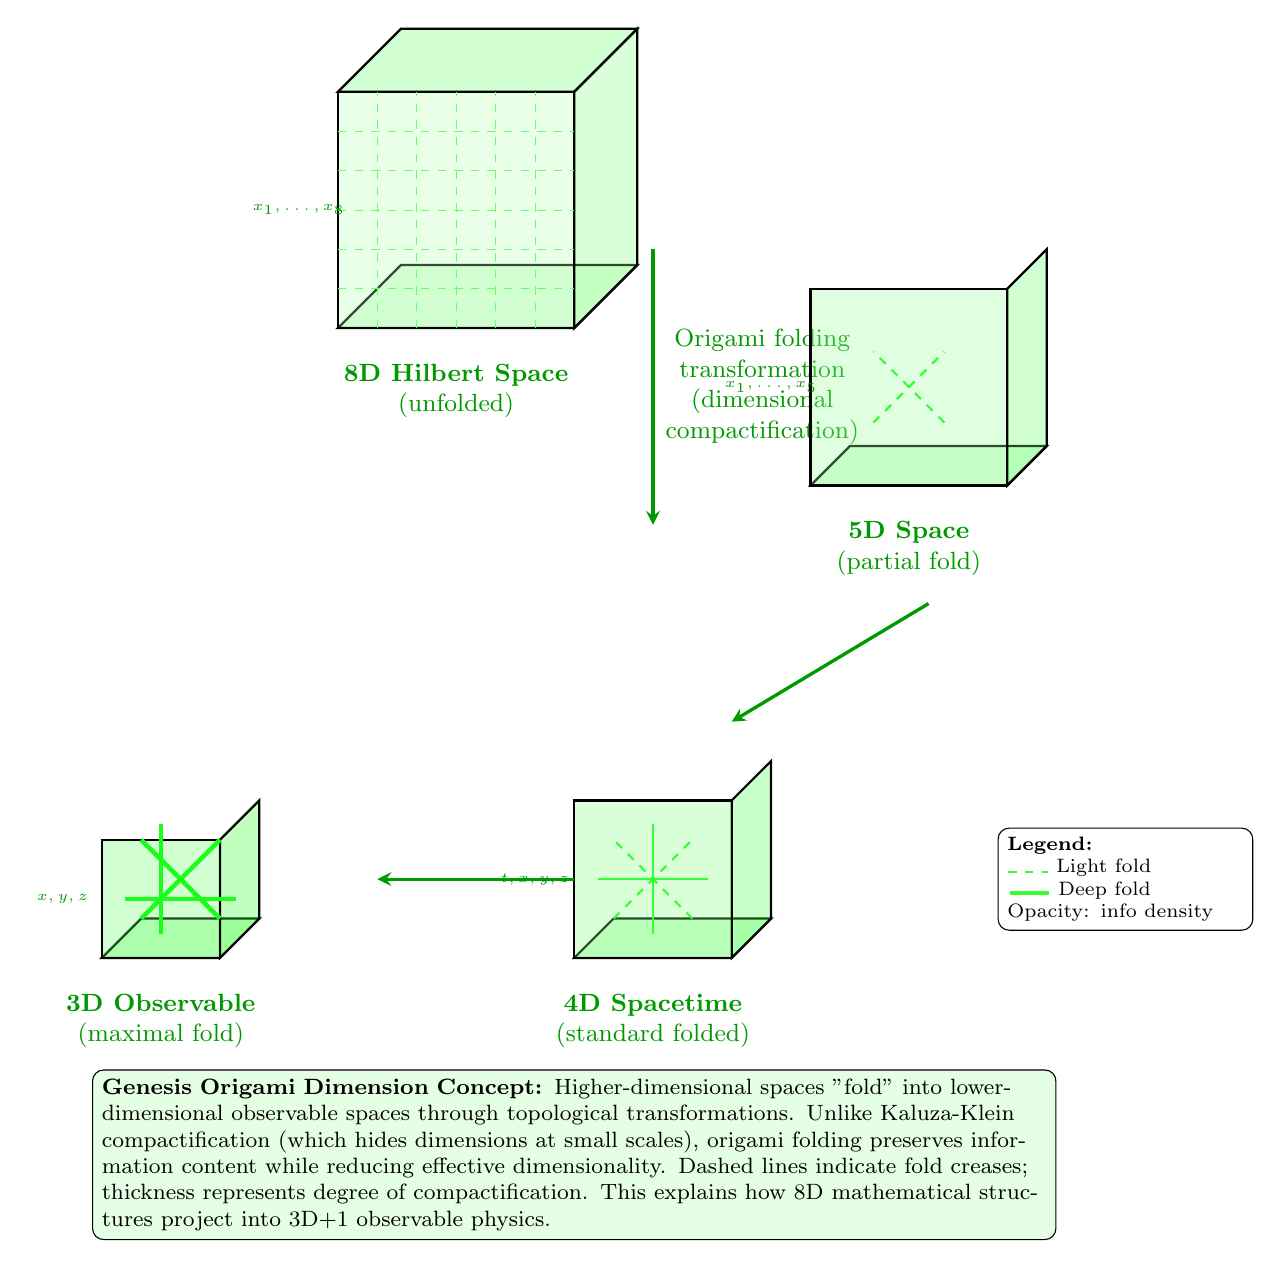
\begin{tikzpicture}[
    scale=1.0,
    dimension/.style={
      draw=black,
      line width=0.8pt,
      fill opacity=0.3
    },
    arrow/.style={
      thick,
      ->,
      >=stealth,
      line width=1.2pt
    },
    label/.style={
      font=\small,
      align=center
    }
  ]

    % 8D space (abstract representation as cube with extra structure)
    \begin{scope}[shift={(0,8)}]
      \draw[dimension, fill=green!40] (0,0) -- (3,0) -- (3.8,0.8) -- (0.8,0.8) -- cycle;
      \draw[dimension, fill=green!50] (3,0) -- (3,3) -- (3.8,3.8) -- (3.8,0.8) -- cycle;
      \draw[dimension, fill=green!30] (0,0) -- (0,3) -- (3,3) -- (3,0) -- cycle;
      \draw[dimension, fill=green!60] (0,3) -- (0.8,3.8) -- (3.8,3.8) -- (3,3) -- cycle;

      % Extra dimension indicators (abstract)
      \foreach \i in {0.5,1.0,1.5,2.0,2.5} {
        \draw[green!60, very thin, dashed] (\i,0) -- (\i,3);
        \draw[green!60, very thin, dashed] (0,\i) -- (3,\i);
      }

      \node[label, text=green!60!black] at (1.5,-0.8) {\textbf{8D Hilbert Space}\\(unfolded)};

      % Dimension labels
      \node[font=\tiny, text=green!60!black] at (-0.5,1.5) {$x_1,\ldots,x_8$};
    \end{scope}

    % Arrow indicating folding transformation
    \draw[arrow, green!60!black] (4,9) -- node[right, label, text width=2.5cm] {
      Origami folding\\transformation\\(dimensional\\compactification)
    } (4,5.5);

    % 5D intermediate (partially folded)
    \begin{scope}[shift={(6,6)}]
      \draw[dimension, fill=green!50] (0,0) -- (2.5,0) -- (3,0.5) -- (0.5,0.5) -- cycle;
      \draw[dimension, fill=green!60] (2.5,0) -- (2.5,2.5) -- (3,3) -- (3,0.5) -- cycle;
      \draw[dimension, fill=green!40] (0,0) -- (0,2.5) -- (2.5,2.5) -- (2.5,0) -- cycle;

      % Folding lines
      \draw[green!80, thick, dashed] (0.8,0.8) -- (1.7,1.7);
      \draw[green!80, thick, dashed] (1.7,0.8) -- (0.8,1.7);

      \node[label, text=green!60!black] at (1.25,-0.8) {\textbf{5D Space}\\(partial fold)};
      \node[font=\tiny, text=green!60!black] at (-0.5,1.25) {$x_1,\ldots,x_5$};
    \end{scope}

    % Arrow to 4D
    \draw[arrow, green!60!black] (7.5,4.5) -- (5,3);

    % 4D spacetime (more folded)
    \begin{scope}[shift={(3,0)}]
      \draw[dimension, fill=green!60] (0,0) -- (2,0) -- (2.5,0.5) -- (0.5,0.5) -- cycle;
      \draw[dimension, fill=green!70] (2,0) -- (2,2) -- (2.5,2.5) -- (2.5,0.5) -- cycle;
      \draw[dimension, fill=green!50] (0,0) -- (0,2) -- (2,2) -- (2,0) -- cycle;

      % More compact folding
      \draw[green!80, thick, dashed] (0.5,0.5) -- (1.5,1.5);
      \draw[green!80, thick, dashed] (1.5,0.5) -- (0.5,1.5);
      \draw[green!80, thick] (1,0.3) -- (1,1.7);
      \draw[green!80, thick] (0.3,1) -- (1.7,1);

      \node[label, text=green!60!black] at (1,-0.8) {\textbf{4D Spacetime}\\(standard folded)};
      \node[font=\tiny, text=green!60!black] at (-0.5,1) {$t,x,y,z$};
    \end{scope}

    % Arrow to 3D
    \draw[arrow, green!60!black] (3,1) -- (0.5,1);

    % 3D observable (maximally folded projection)
    \begin{scope}[shift={(-3,0)}]
      \draw[dimension, fill=green!70] (0,0) -- (1.5,0) -- (2,0.5) -- (0.5,0.5) -- cycle;
      \draw[dimension, fill=green!80] (1.5,0) -- (1.5,1.5) -- (2,2) -- (2,0.5) -- cycle;
      \draw[dimension, fill=green!60] (0,0) -- (0,1.5) -- (1.5,1.5) -- (1.5,0) -- cycle;

      % Highly folded/compact
      \draw[green!90, ultra thick] (0.5,0.5) -- (1.5,1.5);
      \draw[green!90, ultra thick] (1.5,0.5) -- (0.5,1.5);
      \draw[green!90, ultra thick] (0.75,0.3) -- (0.75,1.7);
      \draw[green!90, ultra thick] (0.3,0.75) -- (1.7,0.75);

      \node[label, text=green!60!black] at (0.75,-0.8) {\textbf{3D Observable}\\(maximal fold)};
      \node[font=\tiny, text=green!60!black] at (-0.5,0.75) {$x,y,z$};
    \end{scope}

    % Bottom explanation
    \node[
      draw,
      rounded corners,
      fill=green!10,
      text width=12cm,
      align=left,
      font=\footnotesize
    ] at (3,-2.5) {
      \textbf{Genesis Origami Dimension Concept:} Higher-dimensional spaces "fold" into
      lower-dimensional observable spaces through topological transformations. Unlike
      Kaluza-Klein compactification (which hides dimensions at small scales), origami
      folding preserves information content while reducing effective dimensionality.
      Dashed lines indicate fold creases; thickness represents degree of compactification.
      This explains how 8D mathematical structures project into 3D+1 observable physics.
    };

    % Legend
    \node[
      draw,
      rounded corners,
      fill=white,
      text width=3cm,
      align=left,
      font=\scriptsize
    ] at (10,1) {
      \textbf{Legend:}\\
      \tikz\draw[green!80,thick,dashed] (0,0) -- (0.5,0); Light fold\\
      \tikz\draw[green!80,ultra thick] (0,0) -- (0.5,0); Deep fold\\
      Opacity: info density
    };

  \end{tikzpicture}

  \caption{Conceptual visualization of dimensional folding in the Genesis framework. Higher-dimensional spaces (8D) progressively fold into lower-dimensional observable spaces (3D) through origami-like topological transformations. This differs from traditional compactification: instead of hiding dimensions at small scales, folding reduces effective dimensionality while preserving information content. Fold intensity (line thickness) represents degree of compactification. This mechanism explains how complex higher-dimensional mathematical structures manifest as simpler 3D+1 observable physics without information loss.}
  \abel{fig:dimensional-folding-concept}
\end{figure}
